\chapter{Tests des structures d'égalisation DFVE}

\paragraph{}
Nous devons vérifier expérimentalement deux structures d'égalisation DFVE
(temporelle et fréquentielle). Dans ce chapitre, nous aurons connaissance du
canal de propagation à la réception, sans l'utilisation des pilotes. Nous avons
donc crée un signal OFDM, et modélisé l'effet du canal de propagation. Ensuite,
nous avons testé les deux structures d'égalisation DFVE en connaissant la
réponse du canal, et donc sans algorithme d'estimation des coefficients
complexes (Chapitre suivant). Les codes MATLAB commentés sont disponibles avec ce
rapport.

\section{Création du signal}

\paragraph{}
Nous avons choisi de prendre 4 sous-porteuses avec la première à 2.412 GHz, et
les suivantes espacée de 0.3125MHz afin du simuler 4 sous-porteuses du canal 1
du WIFI en France. Nous avons choisi comme modulation, une $\pi/4$-DPSK dont les
états représentent les chiffres 1, 2, 3 et 4. Nous créerons aléatoirement
un vecteur de ces 4 chiffres, et le modulerons. Nous pouvons voir le diagramme de
constellation sur la Figure ~\ref{QPSK}.

\paragraph{}
\vspace{1\baselineskip}
\begin{figure}[!h]
  \centering
  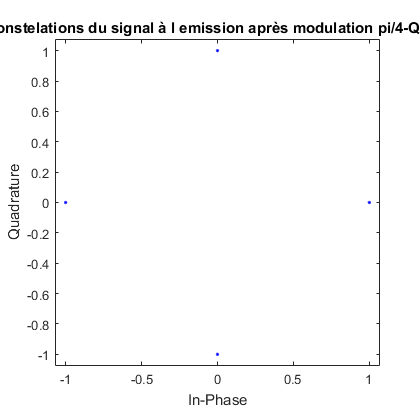
\includegraphics[scale=0.6]{QPSKdep.png}
  \caption{Diagramme de constellation avant l'IFFT }
	\label{QPSK}
\end{figure}
\vspace{10\baselineskip}

\paragraph{}
Ensuite, nous créerons notre signal après en avoir effectué l'IFFT. Nous obtenons le signal visible sur la Figure ~\ref{signal}.

\paragraph{}
\vspace{1\baselineskip}
\begin{figure}[!h]
  \centering
  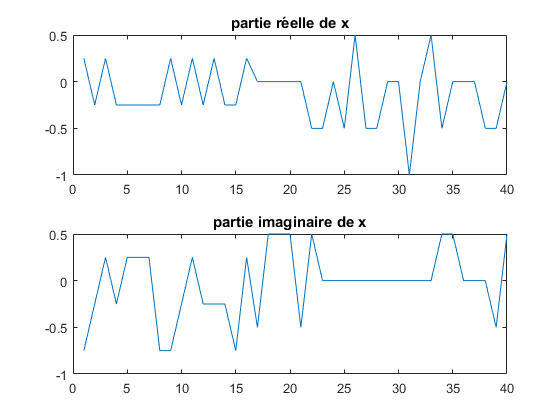
\includegraphics[scale=0.6]{signalSR.png}
  \caption{Signal à la sortie du récepteur }
	\label{signal}
\end{figure}
\vspace{1\baselineskip}

\section{Canal de propagation}
\paragraph{}
Nous avons modélisé la réponse fréquentielle du canal par le filtre d'un canal écho de fonction de transfert $H(f)=1+(0.4+j*0.2)*f^{-1}$. Sur la Figure ~\ref{fonctionT}, nous pouvons voir la réponse en gain et en phase du canal.
\paragraph{}
\vspace{1\baselineskip}
\begin{figure}[!h]
  \centering
  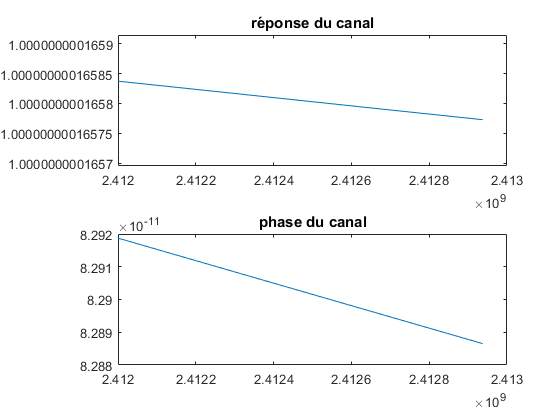
\includegraphics[scale=0.8]{fonctionT.png}
  \caption{Réponse fréquentielle du canal sur la bande du signal OFDM}
	\label{fonctionT}
\end{figure}
\vspace{1\baselineskip}
\paragraph{}
Ensuite nous ajoutons notre signal temporelle à la réponse fréquentielle du
canal par convolution. Puis, nous ajoutons un bruit Gaussien complexe de variance
0.01. Notre signal est ainsi transformé comme nous pouvons le voir sur la Figure
~\ref{ajoutCanal}
\paragraph{}
\vspace{1\baselineskip}
\begin{figure}[!h]
  \centering
  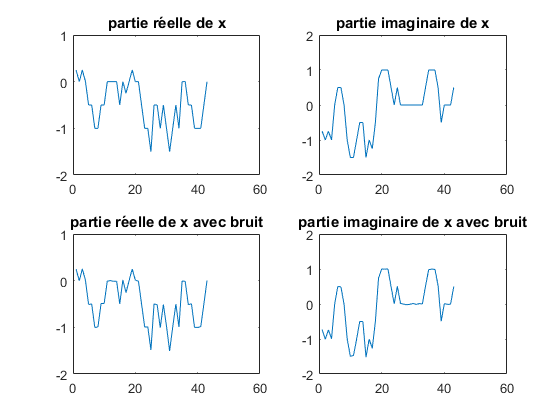
\includegraphics[scale=0.8]{ajoutCanal.png}
  \caption{Signal à l'entrée du récepteur sans bruit et avec bruit}
	\label{ajoutCanal}
\end{figure}
\vspace{1\baselineskip}


\section{Structure fréquentielle DFVE}

\paragraph{}
Pour l'égalisation, nous avons un traitement post-réception afin de compenser
les effets du canal de propagation. Ici, nous avons connaissance de nos
coefficients des matrices $H_0$ et $H_1$ \cite{sujet}, nous n'appliquons donc pas
l'algorithme LMS. Grâce aux deux matrices précédentes, nous avons calculé les
matrices $P_0$ et $P_1$ de la Figure ~\ref{dfveF}.

\paragraph{}
\vspace{1\baselineskip}
\begin{figure}[!h]
  \centering
  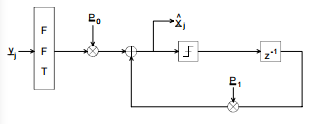
\includegraphics[scale=1]{dfveF.png}
  \caption{Chaîne de réception de la structure fréquentielle DFVE}
	\label{dfveF}
\end{figure}
\vspace{1\baselineskip}
\section{Structure temporelle DFVE}

\paragraph{}
Après notre traitement, on peut voir sur la Figure ~\ref{resultDFVEF}, que les
états du signal à la réception après égalisation correspondent bien aux
constellations du signal de départ. De plus, après démodulation de ces états,
nous avons comparé nos résultats au signal de départ. Pour un faible bruit blanc
Gaussien complexe (variance de 0.01) dans le canal de propagation, nous avons
une erreur de 0\%. Pour un bruit de variance 0.05, nous avons 5\% d'erreurs.

\paragraph{}
\vspace{1\baselineskip}
\begin{figure}[!h]
  \centering
  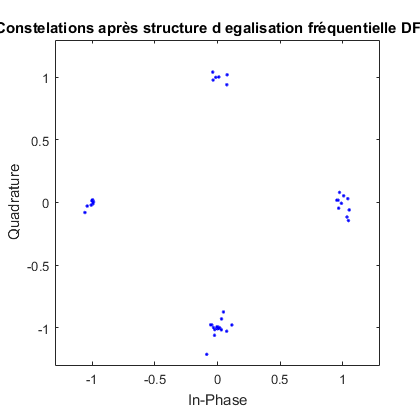
\includegraphics[scale=0.8]{resultDFVEF.png}
  \caption{Diagramme de constellation après égalisation à la réception}
	\label{resultDFVEF}
\end{figure}
\vspace{1\baselineskip}

\section{Structure temporelle DFVE}
\paragraph{}
Avec la structure d'égalisation temporelle DFVE ~\ref{dfveT}, nous avons
exactement les mêmes résultats. Ce qui montre qu'en connaissant exactement la
réponse fréquentielle du canal, les deux structures sont équivalentes. Dans
cette situation, l'avantage de la structure temporelle DFVE est que les matrices
$Q_0$ et $Q_1$ sont triangulaires, ce qui divise par deux la complexité calculatoire.
\paragraph{}
\vspace{1\baselineskip}
\begin{figure}[!h]
  \centering
  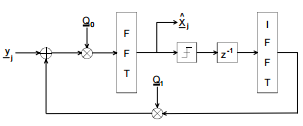
\includegraphics[scale=1]{dfveT.png}
  \caption{Chaîne de réception de la structure temporelle DFVE}
	\label{dfveT}
\end{figure}
\vspace{2\baselineskip}

\paragraph{}
Rappelons, avant de passer à la partie suivante, que nos deux structures sont
équivalentes en résultat car nous avons supposé connaître la réponse
fréquentielle du canal. Mais cela n'est pas vraie en pratique. Le but de la
partie suivante sera de tester une méthode d'estimation des coefficients
complexes des matrices intervenant dans l'égalisation DFVE.

%%% Local Variables:
%%% mode: latex
%%% TeX-master: "../rapport_de_base"
%%% End:
